\chapter{Введение}

\begin{flushright}
\fontsize{10}{12}\selectfont
\textit{Давайте перейдем из эпохи противостояния в эпоху переговоров...}\\
\textit{Ричард Никсон}
\end{flushright}

\label{sec:Chapter0} \index{Chapter0}


В современном мире существует множество задач, которые могут быть решены при помощи технологий искусственного интеллекта. Одной из таких задач является моделирование игр, в которых принимают участие несколько агентов. Это может быть полезным, например, в бизнесе, где агентами могут выступать различные компании. Для них моделирование игр может служить в качестве инструмента прогнозирования рынка, определения стратегий конкуренции и разработки маркетинговой политики. Помимо этого, моделирование игр с несколькими агентами может быть полезным во многих других областях, таких как политика и технологии. В политике моделирование игр может помочь анализировать стратегии и взаимодействия между различными участниками политических процессов. Оно может использоваться для анализа выборов, где различные партии и кандидаты могут выбирать свои стратегии в зависимости от действий своих конкурентов. В технологиях моделирование игр может быть полезно для анализа конкуренции на рынке и разработки новых продуктов и услуг. Компании могут моделировать игры для определения оптимальной стратегии ценообразования на основе поведения конкурентов.


\section{Описание динамических игр двух лиц и мультиагентного обучения с подкреплением}

Пусть у нас есть два игрока, которых мы обозначим как \(A\) и \(B\). Каждый игрок имеет набор возможных стратегий, которые мы обозначим как \(S_A\) и \(S_B\) соответственно. Игрок \(A\) выбирает стратегию \(s_A \in S_A\), а игрок \(B\) выбирает стратегию \(s_B \in S_B\). Выбор стратегии каждым игроком зависит от предыдущих ходов обоих игроков. Выигрыш каждого игрока определяется функцией выигрыша, которую мы обозначим как \(U_A(s_A, s_B)\) для игрока \(A\) и \(U_B(s_A, s_B)\) для игрока \(B\). Эти функции выигрыша зависят от выбранных стратегий обоих игроков. Цель каждого игрока --- выбрать такую последовательность стратегий, которая максимизирует его ожидаемый выигрыш. То есть, игрок \(A\) стремится максимизировать \(U_A(s_A, s_B)\) по всем возможным \(s_A\), а игрок \(B\) стремится максимизировать \(U_B(s_A, s_B)\) по всем возможным \(s_B\).

Что касается MARL, то это подход в машинном обучении при котором агенты обучаются путем взаимодействия друг с другом и с окружающей средой. Каждый агент получает обратную связь от среды в виде награды (англ. reward) или штрафа (англ. penalty) за каждое свое действие. Награда представляет собой меру успеха выполненного действия, а штраф --- меру неудачи.

\begin{figure}[h]
  \centering
  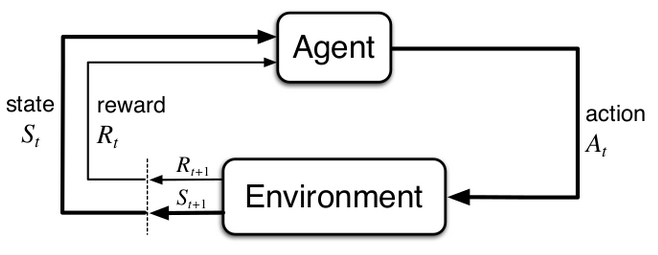
\includegraphics[scale=0.5]{marl.png}
  \caption{Мультиагентное обучение с подкреплением}
\end{figure}

Для моделирования динамических игр с применением обучения с подкреплением и последующего поиска их решений необходимо создать алгоритмы, которые обеспечат взаимодействие агентов в соответствии с заданными правилами и стратегиями. Процесс моделирования можно начать с изучения конфликтной ситуации, которую планируется представить в виде игры и определения предпочтений заинтересованных сторон. В качестве следующего этапа можно рассматривать разработку стратегий и правил. Агенты будут использовать стратегий для достижения своих целей, а правила будут регулировать их поведение. Помимо этого, для эффективного моделирования игр с несколькими агентами необходимо учитывать различные факторы, такие как тип игры, количество и характеристики агентов, возможные исходы при выборе агентами той или иной стратегий. Важно также учитывать возможные изменения в игре и адаптировать стратегии и правила соответствующим образом.


\section{Обоснование выбора темы и актуальность проблемы}

Применение мультиагентного обучения с подкреплением для динамических игр двух лиц является актуальной и перспективной темой для исследования. Приведу несколько аргументов, обосновывающих выбор этой темы и актуальность проблемы:

\begin{enumerate}
    \item Мультиагентное обучение с подкреплением является одним из передовых направлений в области искусственного интеллекта. Изучение применения MARL в динамических играх двух лиц может привести к новым открытиям в разрешении конфликтных ситуации путем переговоров.

    \item В реальных сценариях взаимодействие между агентами играет ключевую роль. Исследование применения мультиагентного обучения с подкреплением в динамических играх двух лиц может помочь разработать новые методы и подходы для эффективного сотрудничества и соперничества между агентами.

    \item Исследование MARL в контексте динамических игр двух лиц может привести к новым применениям в различных отраслях, таких как финансы, экономика, транспорт, робототехника и других. Это может способствовать прогрессу в этих областях и улучшению качества жизни людей.

\end{enumerate}

Мультиагентное обучение с подкреплением является относительно новым направлением исследований в области искусственного интеллекта, которое показало свой потенциал в различных задачах. Мультиагентные системы становятся все более распространенными в различных областях, например, в робототехнике, автономной навигации, финансах, игровой индустрии, бизнесе, политике и других. В таких системах возникает потребность в разработке эффективных методов обучения для агентов, которые позволят им адаптироваться к изменяющимся условиям и достигать высокой производительности в условиях взаимодействия с другими агентами и окружающей средой.


\section{Цель работы и задачи, которые необходимо решить}

Кроме описания различных алгоритмов MARL для решения динамических игр двух лиц, моей целью является разработка новой игры в теории игр --- модифицированной задачи о сделке. Она будет представляться впервые как расширение классической задачи о сделке. В данной игре участники должны соревноваться в некооперативном взаимодействии с целью распределения заданных общих ресурсов между собой. Также собираюсь представить новый подход к распределению ресурсов между участниками, который учитывает влияние участника на переговорный процесс и на основе этого подхода разработать модель искусственного интеллекта, способную решить модифицированную задачу о сделке. Модель будет обучена для поиска оптимальных стратегий и обеспечения эффективной коммуникации между участниками, а также для адаптации к изменяющимся условиям и поведению всех участников.

С помощью математики и искусственного интеллекта хочется создать прикладной инструмент для решения следующих проблем:

\begin{enumerate}
    \item Формализация завершенных конфликтных ситуации, соответствующих описанию данной игры, с целью выяснения на каком этапе стороны не смогли достичь соглашения и каковы были их убытки.

    \item Формализация действующих конфликтных взаимодействий на ранних этапах развития и предложение оптимальных исходов разрешающих такие ситуаций. Доказательство того, что искусственному интеллекту можно доверять разрешение конфликтов.

    \item Моделирование взаимодействии, которые потенциально могут вызвать конфликты в реальной жизни. Учитывая влияние участников на обстановку, их силы, интересы и временной фактор, предложить возможные варианты решении.
\end{enumerate}

Во вступительной части \textbf{первой главы} представлена ознакомительная информация. Глава включает определения MARL и динамических игр. Далее изложены аргументы мотивирующие выбор темы и её актуальность в современных условиях. В завершении главы кратко описывается проблема, которую необходимо решить, и формулируются общие цели дипломной работы.

Во \textbf{второй главе} проведен анализ основных публикаций, посвященных теме игр двух лиц и мультиагентного обучения с подкреплением. Здесь рассмотрены ключевые исследования, описывающие различные подходы и техники, которые сформировали основу современных методов в этой области. Кроме того, дано формальное описание задачи о сделке. Дополнительно сделан подробный обзор существующих подходов к решению этой задачи..

В \textbf{третьей главе} дана формулировка модифицированной задачи о сделке. Там же обоснована необходимость перехода от классической к модифицированной версии задачи о сделке. В заключительной части главы описана мотивация применения методов машинного обучения для решения данной задачи.

\textbf{Четвертая глава} посвящена подробному описанию и сравнению выбранных алгоритмов мультиагентного обучения с подкреплением и их применению к модифицированной задаче о сделке. Обсуждается выбор алгоритмов, процесс обучения и оптимизации, а также обосновывается их применимость для решения данной задачи.

\textbf{Пятая глава} представляет результаты экспериментов, проведенных для оценки эффективности разработанной модели в решении модифицированной задачи о сделке. Здесь описывается среда, в которой проводились эксперименты, и набор данных, использованный для обучения и оценки модели.

Результаты работы обсуждаются в заключительной, \textbf{шестой главе}. В ней также раскрывается прикладная значимость и ценность проведенного исследования. К тому же, данная глава содержит рекомендации по дальнейшему развитию и расширению сферы применения полученных результатов.